\chapter{Application}
\label{ch:Allpication}

The listed algorithms have their theoretical benefits, but they might not be good for real issues. The numeric obstacles require the trade-offs between robustness, stability, and calculation time. The computer memory has limited capacity; systems discretization adds the plant errors. We considered the examples do not have a physical reference system. Now, we try to apply the algorithms on the more ''real'' plant and see the problems that occur. 



	\begin{exam}
		 We consider a dynamical system, which describes a flexible satellite. As known from \cite{SchRC} the continuous-time transfer function has the form  
		\begin{align}
		G(s) = \frac{.036(s + 25.28)}{s^2(s^2 + .0396s + 1)}. 
		\end{align}
		As input we choose the torque on first mass, and as output is set the position $\theta_2$. 
		
		Since we are working with discrete time systems, we discretize it for sample time $T_s = 10^{-3}$  and get the state space description 
		\begin{align}
		\label{eq:Appl:satellite_sys}
		\left( \begin{array}{c | c}
		A & B \\ \hline C & D
		\end{array}\right) = 
		\left(\begin{array}{c c c c | c}
	    1.000  &  0.005  &  0.000  &  0.000 & 1.047\cdot 10^{-13}\\
		0  &  1.000  &  0.001  &  0.000 & 8.333\cdot 10^{-11}\\
		0  &       0  &  1.000  &  0.001 & 2.5\cdot 10^{-7}\\
		0  &       0  & -0.001  &  1.000 & 5\cdot 10^{-4}\\ \hline
        0.362 & 0.072&  0 & 0 & 0
		\end{array}\right). 
	\end{align}
	\end{exam}

In this example, the matrix $D$ is zero, what makes our algorithms not applicable. 
Moreover, the  $D$-part's neglecting is typical: the system output must mostly image the system state and not the known input we send. 

To see more precisely, the input update rule has the form 
\begin{align}
y(t) = C x(t) = C(A x(t) + B u(t)) \text{ for } t = 0, 1,2, \dots, N. 
\end{align}

With other words, the input $u(t)$ begins to impact the output by first iteration, if the matrix $CB$ is not a zero-matrix. That means, that the \textit{relative degree} of the system equals 1. We define it mathematically precise: 
\begin{defi}
	The relative degree of the system $(A, B, C, D)$ is 0 if $D \neq 0$. For $D = 0$ it is the smallest integer $k$ for which $	C A^{k-1} B \neq 0$.
\end{defi} 
Let us denote it with $k^*$. Then the new system we consider can be written as 
\begin{align}
x(t+1) &= A x(t) + B u(t), \\
y(t) &= C x(t) + C A^{k^*} B u(t),  \text{ for } t = k^*, k^* + 1, \dots N. 
\end{align}

We need to put the first iterations away and define a new initial condition $x(k^*)$. The start input condition is then $u(k^*)$. 

For new system all the requirements we considered are satisfied. However, we do not get a better solution for $t = 0, 1, \dots, k^\star - 1$. 


\begin{example}[continued]
	
\textit{For our system the relative degree is 1, as }
	\begin{align}
	CB = 6.038\cdot 10^{-12} \neq 0. 
	\end{align}
	
\textit{We calculate the solution with LQR. Result is illustrated in Figure \ref{img:Appl:Sat_LQR}.}
	
	\begin{figure}[ht]
		\centering
		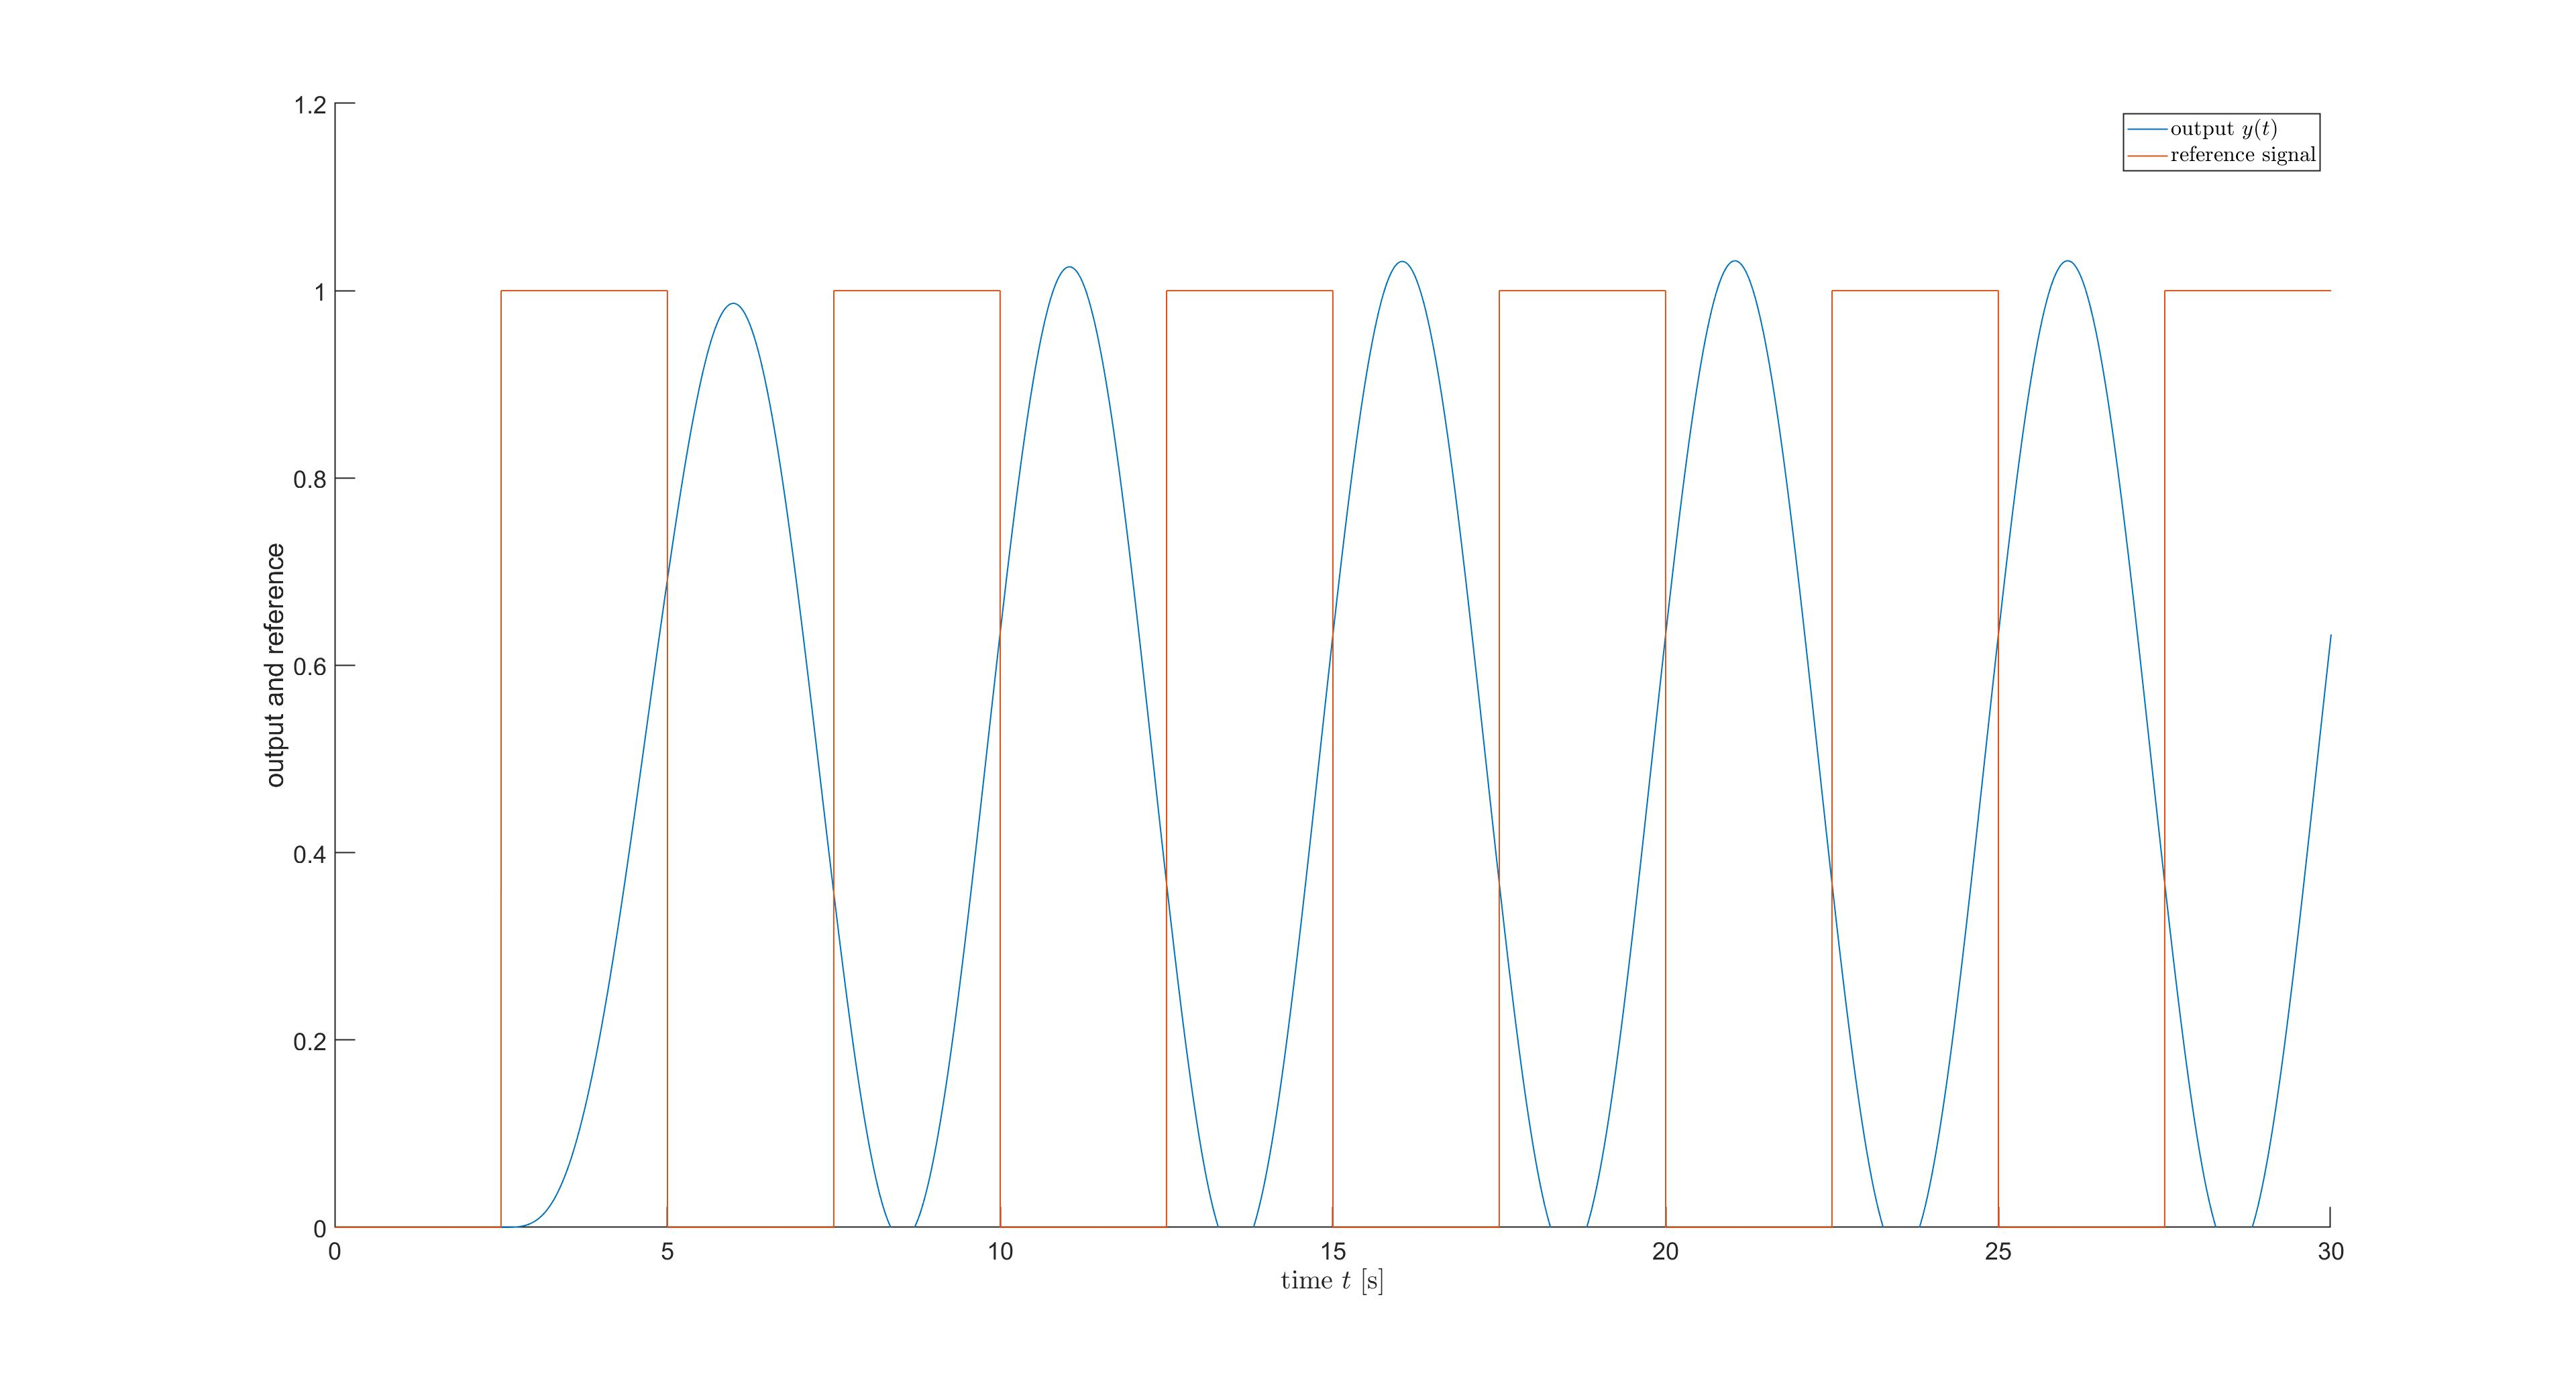
\includegraphics[width=\textwidth]{fig/Ex3_LQR.jpg}
		\caption{LQR Solution for the system \eqref{eq:Appl:satellite_sys}}
		\label{img:Appl:Sat_LQR}
	\end{figure}
	
\textit{It looks like something we can improve. However, for $Ts = 10^{-3}$s we get $N = 10^3$ time steps even for one iteration second. The matrix $G$ has  $10^9$ elements and can not easily be handled.}
\end{example}

	In example \ref{ex:ILC:badIA} the Inverse Model Algorithm is not applicable even for $N = 50$. 
	It means, we need a trade off between the time horizon and robustness.
	However, for real problems the sample times are mostly small, and hence even for one second of the simulation we get huge number for time horizon. Already for SISO system the matrix $G$ will have $N^2$ elements. Our algorithms become unusable for casual applications since they need vast masses of memory.	We can reduce the memory demand by using the sparse matrices: the matrix $G$ is lower triangular, and we can save in this way a lot of space. However, in SDA we need the matrix $G G^{\star}$ to calculate the error $(e_k)_{k\geq0}$, which is not triangular anymore. Can we also here use the advantage of the sparse matrices? 
	
	Let us look at the original system \ref{eq:GP}. At time $t$ the system output equals 
	\begin{align}
	y(t) = C x(t) + D u(t) = C(A^t x_0 + \sum_{\tau = 0}^t A^{t - \tau} u(\tau)) + D u(t).
	\end{align}
	
	Assuming that our model is stable,  we observe the ''past'' terms do not impact our output as mach as the newest ones. We can put this terms in the sum away and get the output 
	\begin{align}
	\t y(t) = C\left(A^t x0 + \sum_{\tau = k}^t A^{t - \tau} u(\tau)\right) + D u(t). 
	\end{align}
	
	The error can be estimated as 
	\begin{align}
	||y(t) - \t y(t)|| &= ||C \sum_{\tau = 0}^k A^{t - \tau} B u(\tau)|| = 
	||C \sum_{\tau = k}^t A^\tau u(t - \tau) B|| \\ \nonumber
	&\leq ||C|| \, ||B|| \sum_{\tau = k}^t||A||^\tau ||u(t - \tau)||.
	\end{align}
	
%	Using the spectral norm, the last inequation results in 
%	\begin{align}
%	||C|| \, ||B|| \sum_{\tau = k}^t||A||^\tau}||u(t - \tau)|| \leq ||C||\, ||B|| \frac{||A||^k - ||A||^t}{1 - ||A||}. 
%	\end{align}
	
	Since our system $(A,B,C,D)$ is assumed to be stable, the last inequation converges for $t \to \infty$.
	
	So, we can reduce our system to 
	\begin{align}
	\t y = \t G + d, 
	\end{align}
	with 
	\begin{align}
	\t G = \begin{pmatrix}
	D  \\
	CB & D \\
	C A B & CB & D\\
	\vdots & \vdots & \vdots & \ddots \\
	C A^{k-1} B & C A^{k-2}B & C A^{k-3}B &\dots& D \\
	0           & C A^{k-1} B & C A^{k-2} B & \dots & CB & D\\
	0 & 0 & C A^{k-1} B & \dots & CAB & CB & D \\
	\vdots & \vdots & \vdots & \ddots & \vdots & \vdots & \vdots & \ddots \\
	0 & 0 & 0 & \dots & C A^{k-1}& C A^{k-2}B& CA^{k-3}B &\dots & D
	\end{pmatrix}.
	\end{align}
	
	Furthermore, for a given tolerance $\varepsilon>0$, this $k$ with the estimation 
	\begin{align}
	\varepsilon \geq ||C||\, ||B|| \frac{||A||^k - ||A||^N}{1 - ||A||} \geq ||C|| \, ||B|| \frac{||A||^k - ||A||^{\t N}}{1 - ||A||}
	\end{align}
	we see, that this $k$ does not change for groving $N$, if the normm $||A|| < 1$ -- this is 
	
	At the beginning of the Chapter \ref{ch:ILCAlg} we assumed the system $(A, B, C, D)$ to be stable. 
	This has a consequence, that for large $p \gg 1$, term $C A^p B \approx 0$. With other words, after some $1<p<N$ we possibly can neglect the terms $C A^k B$ for $k = p, p+1, \dots, N$. Moreover, this number $p$ stays independent on the number of time steps $N$, if $p<N$. 
	
	\begin{theo}
		For the system 
		\begin{align}
		\t y = \t G + d 
		\end{align}
		with 
		\begin{align}
		\t G = \begin{pmatrix}
		D  \\
		CB & D \\
		C A B & CB & D\\
		\vdots & \vdots & \vdots & \ddots \\
		C A^{p-1} B & C A^{p-2}B & C A^{p-3}B &\dots& D \\
		0           & C A^{p-1} B & C A^{p-2} B & \dots & CB & D\\
		0 & 0 & C A^{p-1} B & \dots & CAB & CB & D \\
		\vdots & \vdots & \vdots & \ddots & \vdots & \vdots & \vdots & \ddots \\
		0 & 0 & 0 & \dots & C A^{p-1}& C A^{p-2}B& CA^{p-3}B &\dots & D
		\end{pmatrix},
		\end{align}
		for some $1<p<N$
		the error between the original system output $y$ and $\t y$ can be estimated as 
		\begin{align}
		||y - \t y|| \leq ||C||_1 \, ||B||_1 \frac{||A||_1^p - ||A||_1^{N}}{1 - ||A||_1}. 
		\end{align}
		
		Furthermore, for a given tolerance $\varepsilon>0$, this $p$ does not change for groving $N$, if $p<N$. 
		{\color{red} Abschaetzung ist sehr grob! Man kann sich was besseres ausdenken.}	
		
	\end{theo}
\begin{proof}
	We consider the two lifted matrices $G$ and $\t G$, where$\t G$ is a lower triangular matrix, with terms as in $G$, but where all $C A^k B$ for $k\geq p$ are set to 0 as given above. 
	
	Then the matrix $\t G \t G'$ as well as $\t G \t G^+$ also has less non-zero elements as the original one $G G'$, $G G^+$ -- and we can use the advantage of the sparse matrices. 
	To see the error we get by this reduction, let us consider the difference of the outputs
	\begin{align}
	||y - \t y|| = ||G u + d - \t G u + d || = ||\Delta G u|| \leq ||\Delta G || ||u||, 
	\end{align}
	where 
	\begin{align}
	\Delta G = 
\begin{pmatrix}
	0  \\
	0 & 0 \\
	0 & 0 & 0\\
	\vdots & \vdots & \vdots & \ddots \\
	0 & 0 & 0 &\dots& 0 \\
	C A^{p} B           & 0 & 0& \dots & 0 & 0\\
	C A^{p+1} B & C A^{p} B & 0& \dots &0 & 0 & 0 \\
	\vdots & \vdots & \ddots & \ddots & \vdots & \vdots & \vdots & \ddots \\
	C A^{N-1} B & C A^{N-2} B & \dots & C A^p B& 0& 0 & 0 &\dots & 0
	\end{pmatrix}
	\end{align}
	
	With other words, the matrix $\Delta G$ collects all the ''small'' terms. 
	
	For example, for 1-norm we get 
\begin{align}
||\Delta G||_1  \leq ||C||_1\, ||B||_1 \sum_{l = p}^{N-1}||A||_1^l &= ||C||_1 \, ||B||_1 \frac{||A||_1^p - ||A||_1^N}{1 - ||A||_1} 
\\
&\leq ||C||_1 \, ||B||_1 \frac{||A||_1^p - ||A||_1^{\t N}}{1 - ||A||_1}
\end{align}	
for any $\t N > N$. That means, that even for a longer time horizon we still can use the same $p$ for reduced matrix, without increasing the error. 
\end{proof}
	
With sparse matrices we can reduce the used memory, but it still can be not enough for large $N$. That means, that we need to split our supervectors in the smaller ones, and hope, that the result is not much worse than the original one. 
%
%Let us denote with $\mathtt{N}$ the original time horizon, and with $N$ the part of it, we apply the algorithms on. 
%
%
%	
%	
%	
%	
%	
%	
%
%\begin{example}[contined]
%\textit{Let us use the Steepest descent algorithm, and choose put each time $N =100$ elements into the algorithm. 
%The result is depicted in the Figure \ref{img:Appl:Sat_SDA} We can see, that steepest descent algorithm converges very fast to tracking value, and even for 20 iterations we get perfect tracking. 
%}
%	\begin{figure}[ht]
%	\centering
%	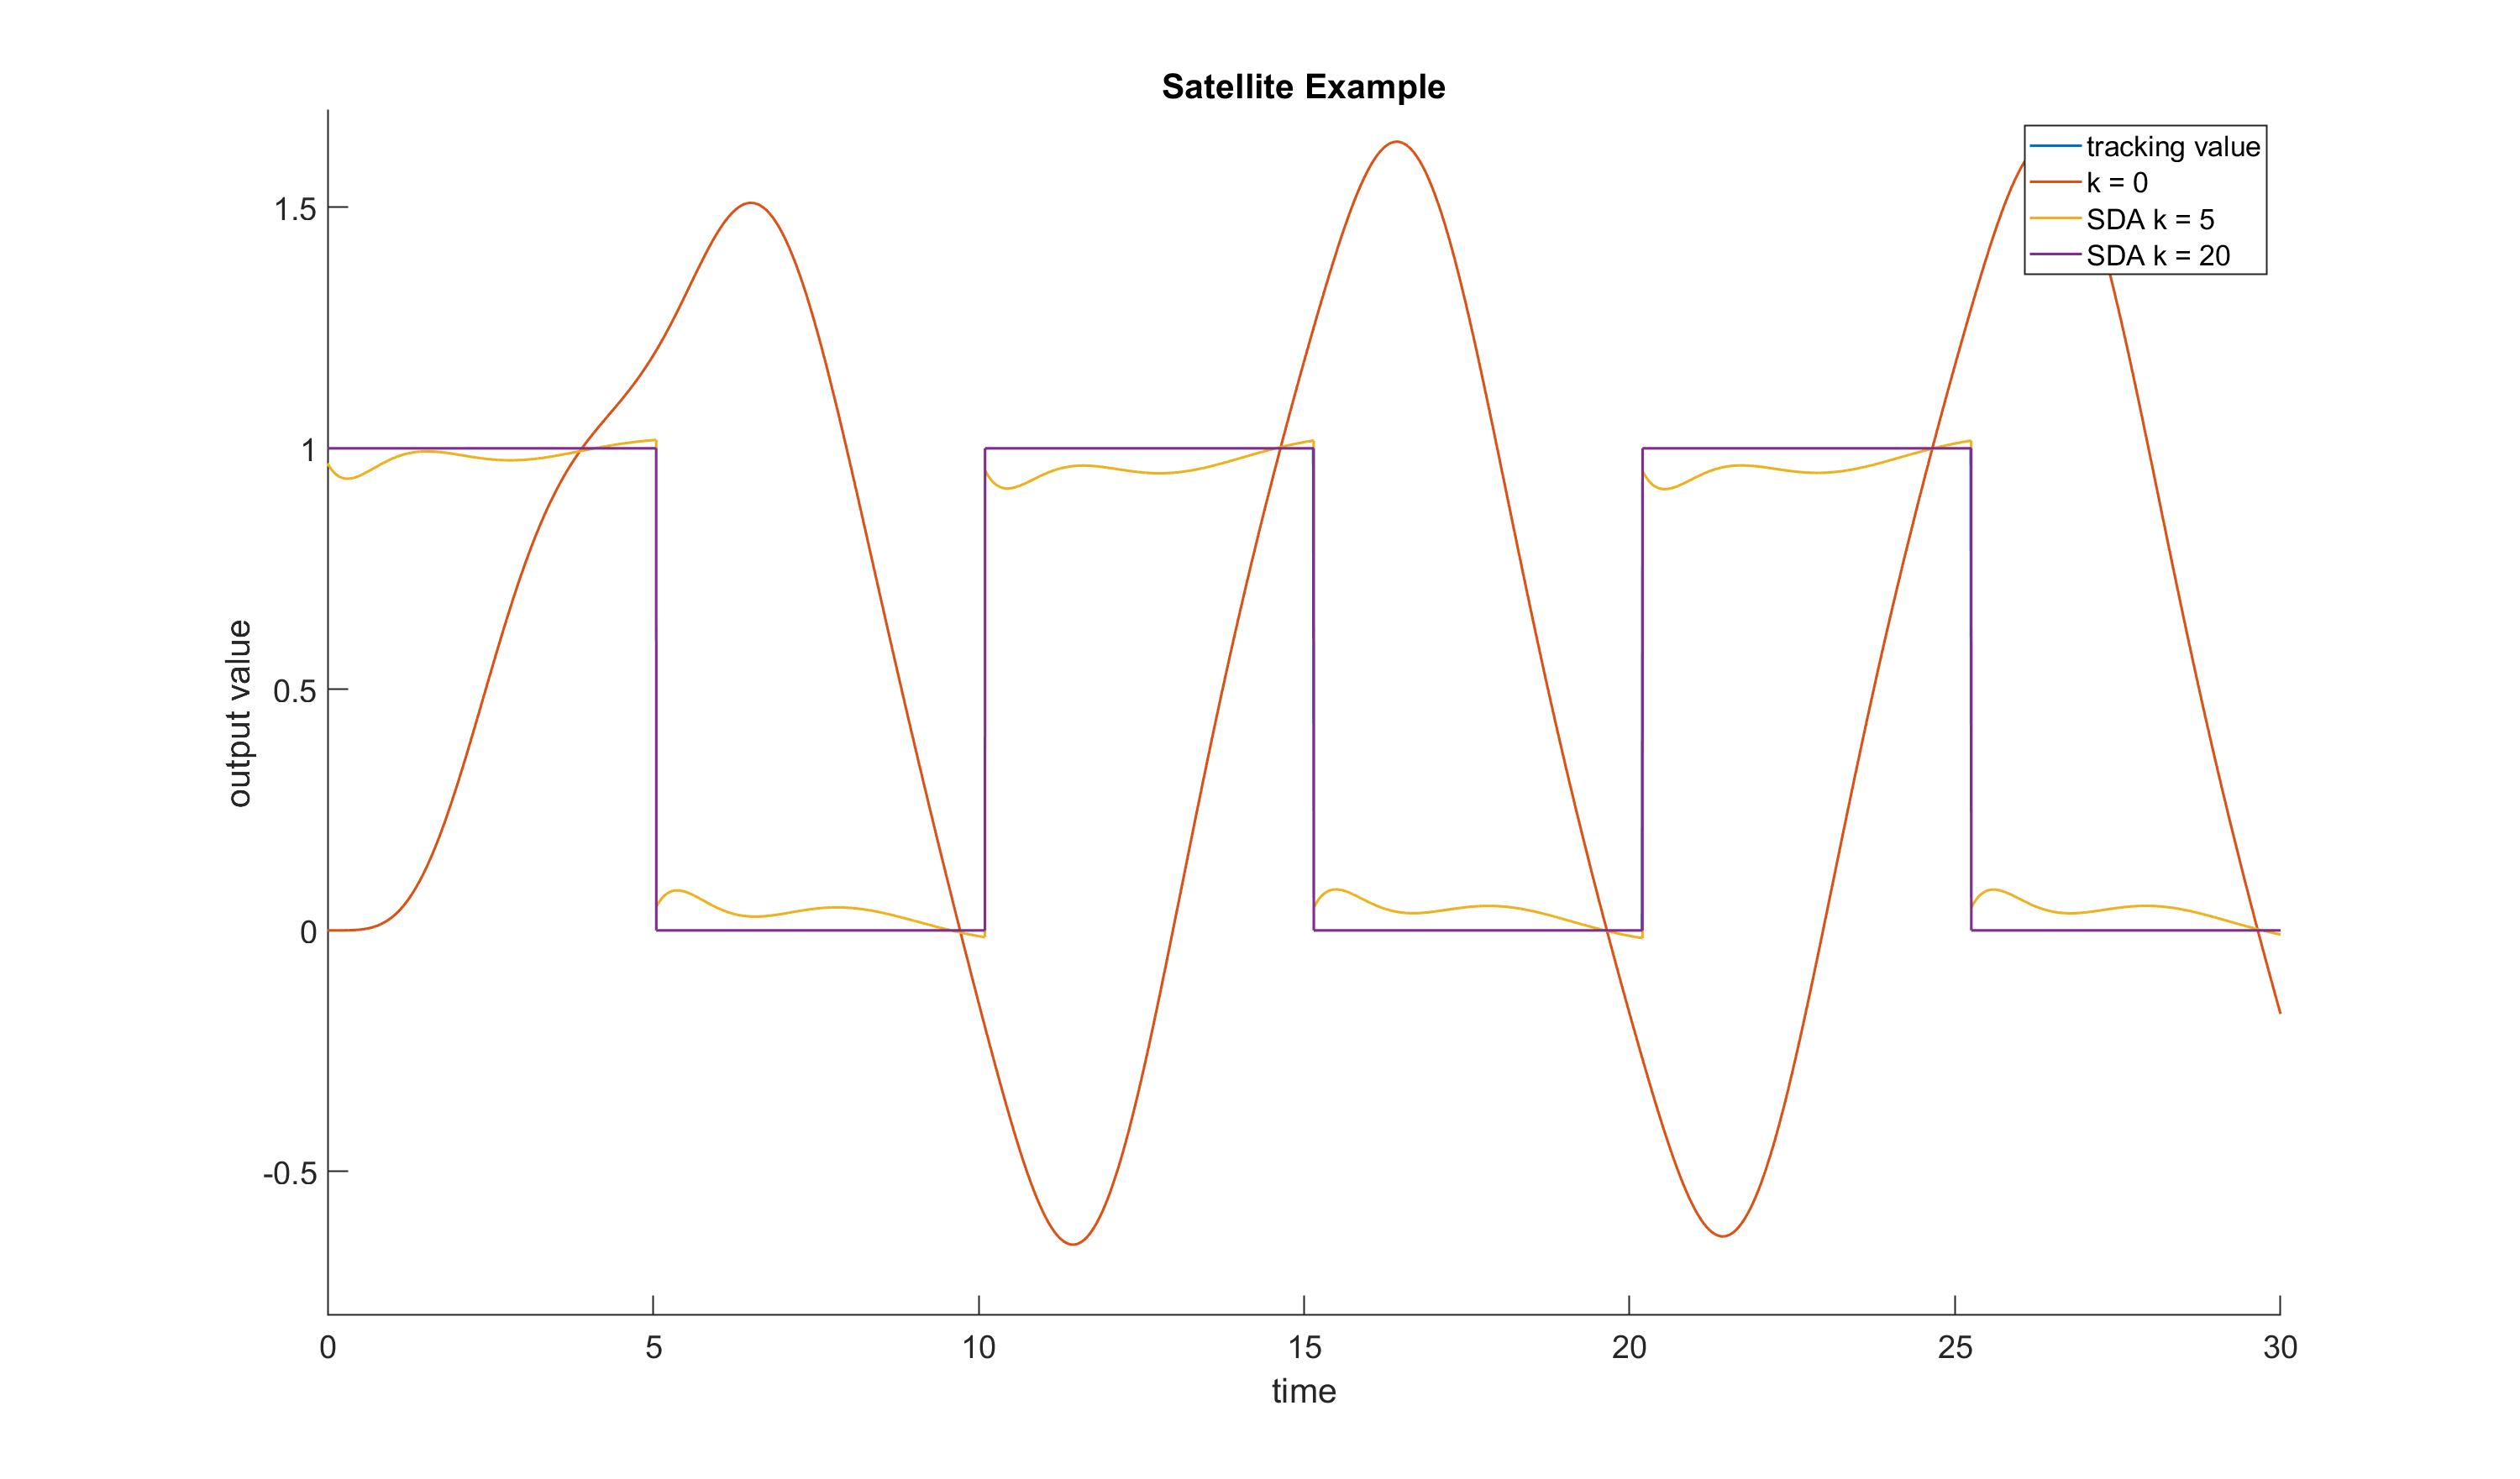
\includegraphics[width=\textwidth]{fig/Satellite_SDA.jpg}
%	\caption{LQR Solution for the system \eqref{eq:Appl:satellite_sys}}
%	\label{img:Appl:Sat_SDA}
%\end{figure}
%
%
%
%\end{example}    

	
	
	